% English Article template created by Vopaaz
\documentclass{article}
\usepackage{geometry}
\geometry{a4paper}
\usepackage{setspace}
\usepackage{enumerate}
\usepackage{enumitem}
\usepackage{hyperref}
\hypersetup{colorlinks,allcolors=black}

\setenumerate[1]{itemsep=0pt,partopsep=2pt,parsep=0pt ,topsep=2pt}
\setitemize[1]{itemsep=0pt,partopsep=2pt,parsep=0pt ,topsep=2pt}
\setenumerate[2]{itemsep=0pt,partopsep=2pt,parsep=0pt ,topsep=2pt}
\setitemize[2]{itemsep=0pt,partopsep=2pt,parsep=0pt ,topsep=2pt}
\setdescription{itemsep=0pt,partopsep=2pt,parsep=0pt ,topsep=2pt}

\usepackage{graphicx}
\usepackage{grffile}
\graphicspath{{../../results/}}

\usepackage{fontspec}

\defaultfontfeatures{%
    RawFeature={%
        % +swsh,
        +calt
    }%
}

\setmainfont{EB Garamond}

%-----------%

\usepackage{amsmath}
\usepackage{amssymb}

\usepackage{multicol}

\usepackage[ruled, linesnumbered]{algorithm2e}

\usepackage{float}

\usepackage{ifthen}
\usepackage{subcaption}

\newcommand{\threefigures}[7][]{
\begin{figure}[H]
	\centering
		\begin{minipage}[t]{0.32\textwidth}
			\centering
			\includegraphics[width=\textwidth]{#2}%
			\subcaption{#3}%
		\end{minipage}
		\begin{minipage}[t]{0.32\textwidth}
			\centering
			\includegraphics[width=\textwidth]{#4}%
			\subcaption{#5}%
		\end{minipage}
		\begin{minipage}[t]{0.32\textwidth}
			\centering
			\includegraphics[width=\textwidth]{#6}%
			\subcaption{#7}%
		\end{minipage}
		\ifthenelse{%
			\equal{#1}{}%
		}{}{%
		\caption{#1}%
		}%
\end{figure}
}

\title{Building a Stock Market Trading Agent with Genetic Algorithm}
\author{YiFan Li\\ZeYuan Yang}
\date{\today}

\begin{document}

\addfontfeatures{RawFeature={+smcp}}
\maketitle
\addfontfeatures{RawFeature={-smcp}}

%-------%

\begin{abstract}

Using algorithms to help financial market traders has been a trend in recent years.
Genetic algorithm is one of the approaches to build an agent
which can suggest buying, selling or holding decisions.
In our paper, we explored different parameter for genetic algorithms,
including survival rate, crossover rate, mutation rate.
Two variants, elitism and chromosome representation are also examined.
We ran the experiment on 5 stock price time series from 2016 to 2018 and compare the results.
It is found that chromosome representation has a critical effect on the result of optimization.
The most flexible one can achieve the best performance on the training dataset,
while the float representation which combines the flexibility and domain knowledge
stand out on the testing dataset.


\end{abstract}

\section{Introduction}

Predicting the future can only happen in science fictions,
but predicting the future trend of some certain time series is feasible.
Time series analysis has a long history, and multiple approaches have been studied.

The most traditional methods are statistical ones such as the well-known ARIMA model.
Although the model is simple, it is still used in recent researches such as \cite{arima-bus-travel}.
Some delicately designed machine learning approaches are also introduced in these years,
varying from relatively simple support vector machine \cite{support-vector-machine}
to complex neural network \cite{time-series-prediction-and-neural-networks}.

The one that receives the most attention among all the time series is probably the stock price.
Firstly, as an essential part of the financial market, the stock market is the apple of investors' eyes.
Not only financial researchers but also individuals and securities companies have
tried their best to analyze the stock price time series and predict its behavior in the future,
to make a fortune.
Secondly, unlike most time series prediction tasks where the output must be exact future values,
only knowing whether the future price will go up or down is already sufficient to make a trading decision.
Therefore, the problem can be simplified thus enabling more ideas and approaches to be applicable.
Thirdly, sufficient financial indexes and trading rules
can serve as domain knowledge to be combined with computer algorithms.

Nowadays, there are numerous financial indexes, and over two hundred different trading rules were
built upon them to suggest buying, selling or holding decisions,
based on historical stock price time series \cite{stock-timing-using-genetic-algorithms}.
Each rule has its rationality and will indicate some features of the target stock.
However, the movement of a stock price is the combined result of a massive number of microeconomic and macroeconomic factors,
which makes it impossible to predict the trend with any index or rule solely.
As Korczak \cite{stock-timing-using-genetic-algorithms} pointed out,
there is no rule consistently outperforming the others.
Therefore, finding the most appropriate way to utilize them becomes the key to the problem.

Although some scholars argue that stock prices follow a random walk pattern,
most experts in this field believe that the prices can be predicted with more than 50 percent accuracy,
with eligible trading rules and reasonable combination \cite{stock-market-prediction-with-multiple-classifiers}.
Plenty of approaches has been examined and we will go through some of them in the literature review.
Noticeably, the genetic algorithm is widely used in related researches.

Genetic algorithm is an adaptive heuristic search method,
inspired by the natural process of genetic evolution.
It can quickly generate high-quality solutions to optimization problems, such as scheduling and shortest path,
and modeling system where randomness is involved, such as the stock market,
by simulating the selection, crossover and mutation procedures in nature
\cite{genetic-algorithm-review-and-application}.

In our paper, we will apply the genetic algorithm to
find the best combination of a set of trading rules, which can help with the buy and sell decisions.
We will dig deeper into a more comprehensive and applicable solution based on the previous works.

\section{Related Work}

We will go through related works about the genetic algorithms first,
then look into its application on the stock time series prediction.

\subsection{Genetic Algorithm}

The genetic algorithm was invented in the early 1970s by John Holland \cite{genetic-algorithm-review-and-application}.
It is based on the mechanics of natural genetic selection.
To conduct GA, a ``chromosome'' must be defined to represent a solution to the problem.
A chromosome is a sequence of alleles, such as a bit.
The genetic features of such representation enable crossover and mutation,
in order to exchange information with each other \cite{an-object-oriented-environment-for-specification}.
A fitness function, which can evaluate the solution, has to be defined as well.
It will be used to select those chromosomes that survive.

The general steps of the genetic algorithm are as follows:
\begin{enumerate}
    \item Initialization. Some chromosomes are randomly generated to form a population.
    \item Selection. During each generation, a proportion of the existing population will be selected
        through a process, where fitter solutions, measured by the fitness function, are more likely to be selected. They are used to generate the population for the next generation.
    \item Reproduction. A second generation population is bred by the previous generation. There are typically
        two genetic operators involved in this step:
        \begin{enumerate}
            \item Crossover. Parent chromosomes are selected from the survivors and their genes are combined in some certain way
                to create a new chromosome.
            \item Mutation. Some genes in some chromosomes are randomly chosen and changed.
        \end{enumerate}
        Generally, the population size is preserved throughout each generation,
        so the selection and reproduction process should counterbalance each other's effect on the number of chromosomes.
    \item Termination. The selection and reproduction are repeated several times until a termination condition has been reached.
        Common termination conditions can be:
        \begin{enumerate}
            \item A solution is found which satisfies a minimum fitness criteria
            \item A fixed number of iteration is reached
            \item The fitness value of the best chromosomes in several successive generations is not improving
        \end{enumerate}
\end{enumerate}

As the genetic algorithm keeps developing, several variants are proposed.
The first one is the chromosome representation.
Traditionally, the chromosome consists of a series of binary bits.
However, in some problem settings, the gene can be a floating-point number
\cite{an-experimental-comparison-of-binary-and-floating}, or even complex data structures like
list or map \cite{helga-a-heterogeneous-encoding}.
The second one is elitism \cite{removing-the-genetics-from-the-standard-genetic-algorithm},
which requires the selection and reproduction to be carefully designed so that
the several best chromosome must be preserved to the next generation.
The third one is the adaptive genetic algorithm \cite{adaptive-probabilities-of-crossover-and-mutation}.
Unlike the traditional ones whose strategy of selection and reproduction is constant,
the possibility of selection, crossover, and mutation will vary in adaptive GA.
The adjustment of these possibilities is related to the current fitness value.
All these variants improved some aspect of the genetic algorithm,
and we will implement some of them in our experiment.


\subsection{Application of GA to Stock Price Prediction}

Given the stock price time series as the original data,
Stephen Leung et al. \cite{a-novel-stock-forecasting-model-based-on-fuzzy-time-series}
modeled it as a fuzzy time series
by converting the percentage of the price change into a fuzzy value.
The fuzzy logic relationship is extracted and classified to form fuzzy logic relationship groups (FLRGs).
FLRGs will then be normalized to get a weight matrix.
Each gene in the chromosome corresponds to a fuzzy value
and the whole chromosome will output a prediction.
The fitness function used in the genetic algorithm is:
$$
\text{RMSE} =
\sqrt{ \dfrac {\sum \limits_{t=1}^{n}\left(\operatorname{actual}(t) - \operatorname{predicted}(t)\right)^2 } {n}}
$$

One technique in their approach is worth mentioning.
The tournament method is used to select survivors in the previous generation.
Several ``tournaments" among a few chromosomes chosen at random from the population are conducted.
The winner of each tournament (the one with the best fitness) is selected for crossover.
Comparing with the traditional approach of directly selecting the good ones from the whole population,
it can improve gene diversity thus prevent GA from being trapped in local optimum
\cite{a-note-on-boltzmann-tournament-selection}.

Applying the fuzzy logic as well, Kuo, Ren Jie and his team \cite{an-intelligent-stock-trading-decision-support-system}
choose to combine genetic and neural networks.
They developed a stock trading system, using GFNN (genetic-algorithm-based fuzzy neural networks)
to build the qualitative model.
The basic model is an FNN (fuzzy neural network), and
the genetic algorithm is used to provide the initial weights and select hyperparameters.
This research and some similar ones utilized the optimization feature of the genetic algorithm,
but put more emphasis on other techniques.

In addition to those combining multiple methodologies to build a complex model
without the help of domain knowledge,
more studies use only GA as the algorithm and take the financial indexes and trading rules into account.
They no longer produce exact value for future time series but provide trading decisions.
As we mentioned before, there are numerous financial indexes,
each summarizing one feature of the stock price time series.
They can be used to build trading rules, which will indicate a decision for buying, selling or holding.
It is the strategy to utilize them that is optimized in those researches.
However, the way they model the problem setting may be slightly different.

Lin Li et al. \cite{the-applications-of-genetic-algorithms-in-stock-market-data-mining}
arbitrarily picked one trading rule, ``the filter rule", and optimize the choice of its parameters.
The fitness function is the profit of trading using its decision.
Comparing with brute force grid search, genetic algorithm saved a lot of running time,
but loses very little precision.
Nevertheless, only using one trading rule limits the model's performance, hence
the profit is still significantly lower than that of a human trader.
Most studies are focused on the way of combining multiple financial indexes.

Fuentu et al. \cite{genetic-algorithms-to-optimise-the-time-to-make-stock-market-investment} selected
three financial indexes, RSI, MACD, and Stochastic Index,
and five of their variants are coded in the algorithm.
The goal is to find the best time to buy stock, indicated by the values of the five index variants.
Each gene in the chromosome represents an interval of the value of a financial index,
and the fitness function is calculated as below:
\begin{enumerate}
\item If there is a period that could match all the financial indexes represented by the chromosome,
    the chromosome's fitness value is the profit of making the buying decision at the start of that period.
\item If there is no such period, the chromosome will not be selected into the next generation.
\end{enumerate}
In the future, when the five financial indexes have the value represented by the best chromosome,
it can be concluded to be the best time to buy a stock.


In some other researches
\cite{genetic-algorithms-for-predicting-the-egyptian-stock-market}
\cite{stock-timing-using-genetic-algorithms}
, the suggestions of trading rules are integrated to give a final trading decision
and such integration is optimized with the genetic algorithm.

Firstly, a set of representative trading rules are selected to examine,
such as Moving Average and Relative Strength Index.
Each gene in the chromosome corresponds to one rule,
with only 1 and 0 as their possible values
representing whether the rule should be considered in the final decision.
The final decision is the voting result of all the rules considered.
On each day in the stock time series, the chromosome will give such a final decision,
and the fitness function is the profit made by these decisions.
After that, a general genetic algorithm can be applied to find the best chromosome.

This approach is intuitive and relatively easy to implement.
Rohit and Kumkum \cite{a-hybrid-machine-learning-system-for-stock-market-forecasting}
take advantage of it and further uses support vector machine
to determine the weight of each rule in the final decision.

Two concerns about this approach are raised, though.
Firstly, the previous experiments are always run on one stock.
Whether this methodology is suitable for more stocks in the market remains a problem
\cite{genetic-algorithms-for-predicting-the-egyptian-stock-market}.
Secondly, whether the resulting chromosome, i.e. combination of trading rules,
remains useful as time goes by is unknown.
Some experts argue that the influence of time is not obvious,
but it still requires examination
\cite{stock-timing-using-genetic-algorithms}.
Our work will be based on the approach introduced above,
try to address these two issues and hopefully find other insights.

\section{Approach}

\subsection{Problem Setting Specification}

Similar to \cite{genetic-algorithms-for-predicting-the-egyptian-stock-market}
and \cite{stock-timing-using-genetic-algorithms},
we will setup our problem setting as follows:
\begin{itemize}
    \item Given a historical stock price time series in the past $n$ periods, $P_t=\left[p_{t-n}, p_{t-n+1}, \cdots, p_{t-1}\right]$,
          where $t$ represents the present,
    \item and a set of $k$ trading rules suggesting ``buy", ``sell" or ``hold" action based on the time series\\
          $R=\{r_1, r_2, \cdots, r_k\}, \forall r_i(P_t) \rightarrow s_i \in \{\text{sell}, \text{buy}, \text{hold}\}$,
    \item design an agent $A$ who can integrate all the rules to make a final decision\\
          $A(R(P_t)) \rightarrow d_t \in \{\text{sell}, \text{buy}, \text{hold}\}$,
    \item that can generate profit in the following $m$ period,
          which can be calculated as $\sum \limits_{t=0}^{m} p_{t}^{\text{sell}} - p_{t}^{\text{buy}}$,\\
          $p_{t}^{\text{sell}} = \left\{
              \begin{array}{ll}
                  p_t \quad & \text{if} A(R(P_t)) = \text{sell} \wedge A \text{ currently holds the stock} \\
                  0 \quad   & \text{otherwise}
              \end{array}\right.,\\
              p_t^{\text{buy}} = \left\{
              \begin{array}{ll}
                  p_t \quad & \text{if} A(R(P_t)) = \text{buy} \wedge A \text{ currently not holds the stock} \\
                  0 \quad   & \text{otherwise}
              \end{array}
              \right.$
\end{itemize}

As examining only one stock is not representative enough,
we will experiment on five stocks and take their average result.
Additionally, because the maximum possible benefit varies for different stock price time series,
it is unwise to compare the absolute value of profit directly.
The benchmark of our evaluation is an agent who can ``predict the future".
It knows the whole time series and makes the decision based on it,
$A'(P_m, t) \rightarrow d'_t$,
which can be implemented with the following trivial algorithm.

\begin{algorithm}[H]
    \KwData{prices}
    \KwData{today}
    \SetKwData{prices}{prices}
    \SetKwData{today}{today}
    \KwResult{decision}

    \uIf{$\prices[\today+1] > \prices[\today]$}{
        \Return{buy}\;
    }\uElseIf{$\prices[\today+1] < \prices[\today]$}{
        \Return{sell}\;
    }\Else{
        \Return{hold}\;
    }
    \caption{Benchmark Agent}
\end{algorithm}

In all, the evaluation of the agent will be
$
\dfrac{\sum \limits_{i=1}^{5}
\dfrac{
    \operatorname{Profit}_i(\text{genetic agent})
}{
    \operatorname{Profit}_i(\text{benchmark agent})
}}{5}$, where $i$ represents different stocks, and the goal is to maximize it.


\subsection{Genetic Algorithm}

\subsubsection{Chromosome Representation}

In our experiment, each gene in the agent's chromosome will be a number
\footnote{In the complex representation variant,
a part of the gene will be a number.
See section \ref{subsubsec-variants} for detail.}
corresponding to one trading rule.
It will be used as the weight to take an average on the trading rules' decision.
The decisions can be considered as:
\begin{itemize}
    \item Buy $\rightarrow$ 1
    \item Sell $\rightarrow$ -1
    \item Hold $\rightarrow$ 0
\end{itemize}

After that, a positive weighted average will result in a Buy decision,
while a negative one will lead to a Sell decision outputted by the agent.

\subsubsection{Genetic Operators}

Various implementations for genetic algorithm operators are proposed in previous works.
For example, there are trivial highest-score and tournament method\cite{a-note-on-boltzmann-tournament-selection} selection,
single-point, k-point and uniform crossover\cite{genetic-algorithm-review-and-application}, etc.
Therefore we considered it necessary to describe
our implementation of the genetic operators explicitly.

We applied the basic highest-score selection,
which selects a percentage of agents with the highest score to go to the reproduction process.

In the crossover phase, a percentage of agents who passed the selection will be chosen.
They will act as parents, producing new agents, but they will not go to the next generation.
The children and those who are not selected as parents will go to the mutation phase.
When generating a new agent, uniform crossover will run repeatedly,
until the total number of the agent is the same as the original.
Uniform crossover, to be more specific, means that each gene in the children's chromosome
is chosen from either parent with equal probability.

During mutation, a percentage of the agents will be chosen to mutate,
the others will remain unchanged.
Each gene in the chromosome of mutating agents will have a 50\% chance to be reset as a random one.

\subsubsection{Variants}\label{subsubsec-variants}

Chromosome representation\cite{genetic-algorithm-review-and-application} is applied in our experiment.
Besides the bit representation used in \cite{genetic-algorithms-for-predicting-the-egyptian-stock-market}
and \cite{stock-timing-using-genetic-algorithms}
where all the genes are either 0 or 1,
they can also be:
\begin{itemize}
    \item A floating number ranging from 0 to 1
    \item A tuple, whose first element is a floating number and second element is a list,
    containing the parameters for the financial rule
\end{itemize}

As mentioned before, the genes will be used as weights to take an average on the rules output.
The bit, the float and the first element in the tuple, respectively, will be of this usage.
The second element of the tuple representation is used to configure the financial rules,
who have some adjustable parameters, but set to a default value based on financial researches
in the bit and float representation.
The more complex the chromosome representation is, the more flexible it can integrate all information.
However, the searching space will be larger.

Elitism is also implemented in the experiment.
Note that in the basic procedures described above,
the best agent may be selected as a parent, therefore, will not proceed to the next phase,
or its gene could be changed in the mutation phase.
If a rate of elitism is specified, a copy of that percentage of the best agents will be directly used
as the agents for the next generation.
The numbers of agents generated by crossover will correspondingly adjust so that the total amount of
agent stays constant between each generation.
With this technique, it can be guaranteed that the best agent will only improve as it evolves.

\subsection{Experiment Plan}

The possible configurations in our experiment are:
\begin{itemize}
    \item survival rate
    \item crossover rate
    \item mutation rate
    \item elitism rate
    \item chromosome representation
\end{itemize}

We will try different combinations of these parameters/choices and compare their results.
Some fixed hyper-parameters are:
\begin{itemize}
    \item population: 15
    \item total training epoch: 8
\end{itemize}

We will split the data into two parts, from 2016--03--01\textasciitilde 2017--12--29 as the training dataset,
and use the data from 2018--01--02\textasciitilde 2018--12--28 as the test dataset.
The genetic optimization will only run on the train set,
and the final population will be applied to the test set to evaluate their performance.
This idea is borrowed from machine learning,
that a model with high performance may not be accurate on unseen data.
We can test the final agent's ability to generalize with this approach.

\subsection{Other Technical Details}

\subsubsection{Data Preparation}

The open, high, low, close price and trading volume
of the five randomly chosen stocks, CMS, MKC, MMP, THS, and XEL,
between 2016--01--04 and 2018--12--31 are pulled from \href{https://www.alphavantage.co/}{Alpha Vantage}.
They will be used as our dataset.
The data quality is good, therefore no further preprocessing is required.

\subsubsection{Programming Language and Packages}

We chose Python as the programming language it is simple.
Its Pandas and Numpy packages also significantly simplify array and matrix computation.
There are also various modules providing a fundamental framework for genetic algorithm,
however, we decide not to use them and build the genetic algorithm related modules from scratch,
because we want to know the exact details of every single line of code
in the genetic algorithm.

\subsubsection{Trading Rules Specification}

As the financial trading rules are verbose to explain and the details are off-topic,
we will specify them in section \ref{section-appendix-financial-rules}, appendix.

\section{Results and Analysis}

We tracked the performance of the best agent and
the population average of each generation in the training phase.
The best and average performance of the final generation in the testing phase is also recorded.
In the following several sections,
we will interpret the effect of the genetic operators and variants
by looking at the figures which depict the training process and the testing result.
The lines in the figures are explained as follows:
\begin{itemize}
    \item Blue line: best agent in each generation (epoch), performance on the train set
    \item Orange line: population average in each generation (epoch), performance on the train set
    \item Green dashed line: best agent in the final population, performance on the test set
    \item Orange dashed line: the average of the final population, performance on the train set
\end{itemize}

Although all the information is demonstrated,
we would like to focus on the training performance in the following sections first.
Comments on the testing performance will be made in section \ref{subsection-generalization}.

\subsection{Survival rate}

The survival rate is the percentage of well-performed agents
who can go to the reproduction procedures.
The effect of the survival rate is analyzed in this section by controlling the following parameters:
\begin{itemize}
    \item crossover rate: 0.75
    \item mutation rate: 0.1
    \item elitism: off
\end{itemize}

The following figure
shows the experiment result of applying different survival rate
in the bit representation.

\threefigures[Bit representation]
{bit-15-agent-param-0.4-0.75-0.1.png}
{Survival rate: 0.4}
{bit-15-agent-param-0.5-0.75-0.1.png}
{Survival rate: 0.5}
{bit-15-agent-param-0.6-0.75-0.1.png}
{Survival rate: 0.6}

All the best performers reached a performance of about 0.08 in about 5 generations.
The population average converges to the best agent gradually and is fairly close in the final generation.
Such convergence happens somewhat faster when the survival rate is 0.4 but it is not significant.
In all, no prominent difference can be identified in the figures.

However, the situation differs a lot in the float and tuple representation, as shown below.

\threefigures[Float representation]
{real-15-agent-param-0.4-0.75-0.1.png}
{Survival rate: 0.4}
{real-15-agent-param-0.5-0.75-0.1.png}
{Survival rate: 0.5}
{real-15-agent-param-0.6-0.75-0.1.png}
{Survival rate: 0.6}

\threefigures[Tuple representation]
{complex-15-agent-param-0.4-0.75-0.1.png}
{Survival rate: 0.4}
{complex-15-agent-param-0.5-0.75-0.1.png}
{Survival rate: 0.5}
{complex-15-agent-param-0.6-0.75-0.1.png}
{Survival rate: 0.6}

When survival rate is 0.4, the population average converges to the best agent,
and is almost the same in the final population.
Such convergence means that the genetic diversity of the population is really low,
all agents are likely to have highly similar chromosomes.
However, when the survival rate is 0.5, the tuple representation,
maintains a good gene diversity even in the final epoch.
The same goes for a 0.6 survival rate for both float and tuple representation.

Although a higher survival rate improves the diversity of the gene pool,
it set back the efficiency of optimization.
When survival rate is 0.6 in float representation,
hardly does the best agent perform better.
The best agent in tuple representation even perform worse than the initial best,
making the whole genetic algorithm approach almost meaningless.

\subsection{Crossover Rate}

The crossover rate is the percentage of agents who are used to generate new agents.
The effect of the crossover rate is analyzed in this section by controlling the following parameters:
\begin{itemize}
    \item survival rate: 0.6
    \item mutation rate: 0.1
    \item elitism: off
\end{itemize}

The following figure demonstrates the experimental results using the bit chromosome representation.

\threefigures[Bit representation]
{bit-15-agent-param-0.6-0.25-0.1.png}
{Crossover rate: 0.25}
{bit-15-agent-param-0.6-0.5-0.1.png}
{Crossover rate: 0.5}
{bit-15-agent-param-0.6-0.75-0.1.png}
{Crossover rate: 0.75}

All the average performance grows fast and smoothly,
but there are a lot of horizontal lines in the performance of the best agents.
Changing the crossover rate does not help to change this situation in bit representation,
but it makes a slight difference in float and tuple representation as shown by the following figures.

\threefigures[Float representation]
{real-15-agent-param-0.6-0.25-0.1.png}
{Crossover rate: 0.25}
{real-15-agent-param-0.6-0.5-0.1.png}
{Crossover rate: 0.5}
{real-15-agent-param-0.6-0.75-0.1.png}
{Crossover rate: 0.75}

\threefigures[Tuple representation]
{complex-15-agent-param-0.6-0.25-0.1.png}
{Crossover rate: 0.25}
{complex-15-agent-param-0.6-0.5-0.1.png}
{Crossover rate: 0.5}
{complex-15-agent-param-0.6-0.75-0.1.png}
{Crossover rate: 0.75}

When the crossover rate is low, there are a lot of horizontal lines for the best agent as well.
However, with a crossover rate of 0.75, the best agent gets updated in almost every generations,
even though the improvement is not significant, if not deterioration.
A high crossover rate also prevents the population average from improving fast.

In all, the crossover rate does not have a clear pattern of affecting the genetic optimization in our problem.
It helps ensure the updating of the best agent in each generation,
but whether such an update is positive or negative cannot be guaranteed.

\subsection{Mutation Rate}

The mutation rate is the percentage of agents whose genes will be randomly modified.
The effect of mutation rate is analyzed in this section by controlling the following parameters:
\begin{itemize}
    \item survival rate: 0.6
    \item crossover rate: 0.75
    \item elitism: off
\end{itemize}

The following figure demonstrates the experimental results using the bit and float chromosome representation.

\threefigures[Bit representation]
{bit-15-agent-param-0.6-0.75-0.1.png}
{Mutation rate: 0.1}
{bit-15-agent-param-0.6-0.75-0.2.png}
{Mutation rate: 0.2}
{bit-15-agent-param-0.6-0.75-0.3.png}
{Mutation rate: 0.3}

\threefigures[Float representation]
{real-15-agent-param-0.6-0.75-0.1.png}
{Mutation rate: 0.1}
{real-15-agent-param-0.6-0.75-0.2.png}
{Mutation rate: 0.2}
{real-15-agent-param-0.6-0.75-0.3.png}
{Mutation rate: 0.3}

When the mutation rate is low, the best performance and the average performance of both representations
are all monotonically increasing.
However, when the mutation rate is higher, the performance starts to fluctuate.
A mutation rate of 0.3 in float representation even causes the best agent's performance to deteriorate.

Such a pattern of fluctuation seems to be reversed in the tuple representation, see the figure below.

\threefigures[Tuple representation]
{complex-15-agent-param-0.6-0.75-0.1.png}
{Mutation rate: 0.1}
{complex-15-agent-param-0.6-0.75-0.2.png}
{Mutation rate: 0.2}
{complex-15-agent-param-0.6-0.75-0.3.png}
{Mutation rate: 0.3}

With a low mutation rate, the fluctuation is more severe than that with a high mutation rate.
It can be observed that with a mutation rate of 0.3,
the average of population performance has a stable monotonic increasing trend.

\subsection{Elitism}

Elitism ensures a percentage of best agents go to the next generation unmodified.
The effect of elitism is analyzed in this section by controlling the following parameters:
\begin{itemize}
    \item survival rate: 0.6
    \item crossover rate: 0.75
    \item mutation rate: 0.1
\end{itemize}

The following figure demonstrates the experimental results using the bit representation.

\threefigures[Bit representation]
{bit-15-agent-param-0.6-0.75-0.1.png}
{Elitism rate: 0}
{bit-15-agent-param-0.6-0.75-0.1-0.1.png}
{Elitism rate: 0.1}
{bit-15-agent-param-0.6-0.75-0.1-0.2.png}
{Elitism rate: 0.2}

There is no significant difference between different elitism rates.
Even without the elitism, the best/average performance are both monotonically increasing.
And in the final generation, the performance of the best agent and population average
are fairly close.

The following figure demonstrates the result of the float representation.

\threefigures[Float representation]
{real-15-agent-param-0.6-0.75-0.1.png}
{Elitism rate: 0}
{real-15-agent-param-0.6-0.75-0.1-0.1.png}
{Elitism rate: 0.1}
{real-15-agent-param-0.6-0.75-0.1-0.2.png}
{Elitism rate: 0.2}

With a high elitism rate of 0.2, the average performance quickly converges to the best performance.
It shows that elitism could decrease the gene diversity.
However, this pattern is not observed in the tuple representation.

\threefigures[Tuple representation]
{complex-15-agent-param-0.6-0.75-0.1.png}
{Elitism rate: 0}
{complex-15-agent-param-0.6-0.75-0.1-0.1.png}
{Elitism rate: 0.1}
{complex-15-agent-param-0.6-0.75-0.1-0.2.png}
{Elitism rate: 0.2}

The divergence of the population average and best agent's performance seems to be not
accelerated by the increasing elitism rate.
On the other hand, the fluctuation of performance without elitism no longer exists
with elitism adopted, which is a trivial result of the concept of elitism itself.

\subsection{Chromosome Representation}

The figures listed in the previous sections can be used to
compare the three chromosome representations we implemented.
Therefore, we will not display them here again.

The bit representation has only limited possible genes.
The search space of float representation, however, is infinite.
The tuple representation is even larger than that of float representation,
and it dropped the support of domain knowledge.
The underlying rules no longer use the generally accepted parameters,
instead, the genetic algorithm is in charge of optimizing them so that they
can ideally fit the current stock price series even better.

Such a difference is the reason why the same genetic algorithm parameters show different patterns.
With a limited search space, the bit representation itself tends to
have an undiversified gene pool.
Smaller survival rate and larger mutation rate will help to introduce diversity in the gene pool,
hence improve the overall performance.
On the contrary, the float and tuple representation are more unstable.
Excessively aggressive crossover and mutation will deteriorate the optimization by disrupting the
survival of high-quality genes.
A moderate elitism rate, on the other hand, will protect the good genes, therefore, improving the
result of the genetic algorithm.
The 0.1 elitism rate of tuple representation most clearly demonstrates that.

Another interesting phenomenon of different representations is the final training best and average.
The following table listed the three configurations that result in the best agents,
and the three configurations that result in the worst agents in the training phase.

\begin{table}[H]
    \centerline{
    \begin{tabular}{ccccc|cc}
    Representation & Survival & Crossover & Mutation & Elitism & Training Best & Training Avg \\\hline
    tuple          & 0.5      & 0.75      & 0.1      &         & 0.09          & 0.07         \\
    tuple          & 0.6      & 0.75      & 0.1      & 0.2     & 0.088         & 0.072        \\
    tuple          & 0.6      & 0.75      & 0.1      & 0.1     & 0.086         & 0.069        \\\hline
    bit            & 0.6      & 0.5       & 0.1      &         & 0.057         & 0.048        \\
    tuple          & 0.6      & 0.75      & 0.3      &         & 0.057         & 0.031        \\
    tuple          & 0.6      & 0.75      & 0.1      &         & 0.052         & 0.04
    \end{tabular}}
    \caption{Top and Bottom 3 Configurations for the Training Best}
\end{table}

Interestingly, the tuple chromosome dominates the top three,
while two of the bottom three are also tuple chromosomes.
As mentioned before, the tuple representation has the most flexibility
for fitting the characteristics of a certain stock price time series.
On the other hand, if it stuck in a local optimum, or the gene pool is disrupted by the aggressive mutation,
or not enough number of epochs is conducted,
the flawed trading rule parameters will prevent the rules from outputting an effective decision.
Therefore the performance of the agent is certainly limited.

\subsection{Generalization}\label{subsection-generalization}

In the previous figures, the testing performance in each experiment is depicted.
To get a more clear view of their relationship with the training performance,
we can plot all experiment results on a scatter plot as follows.

\begin{figure}[H]
    \centering
        \begin{minipage}[t]{0.49\textwidth}
            \centering
            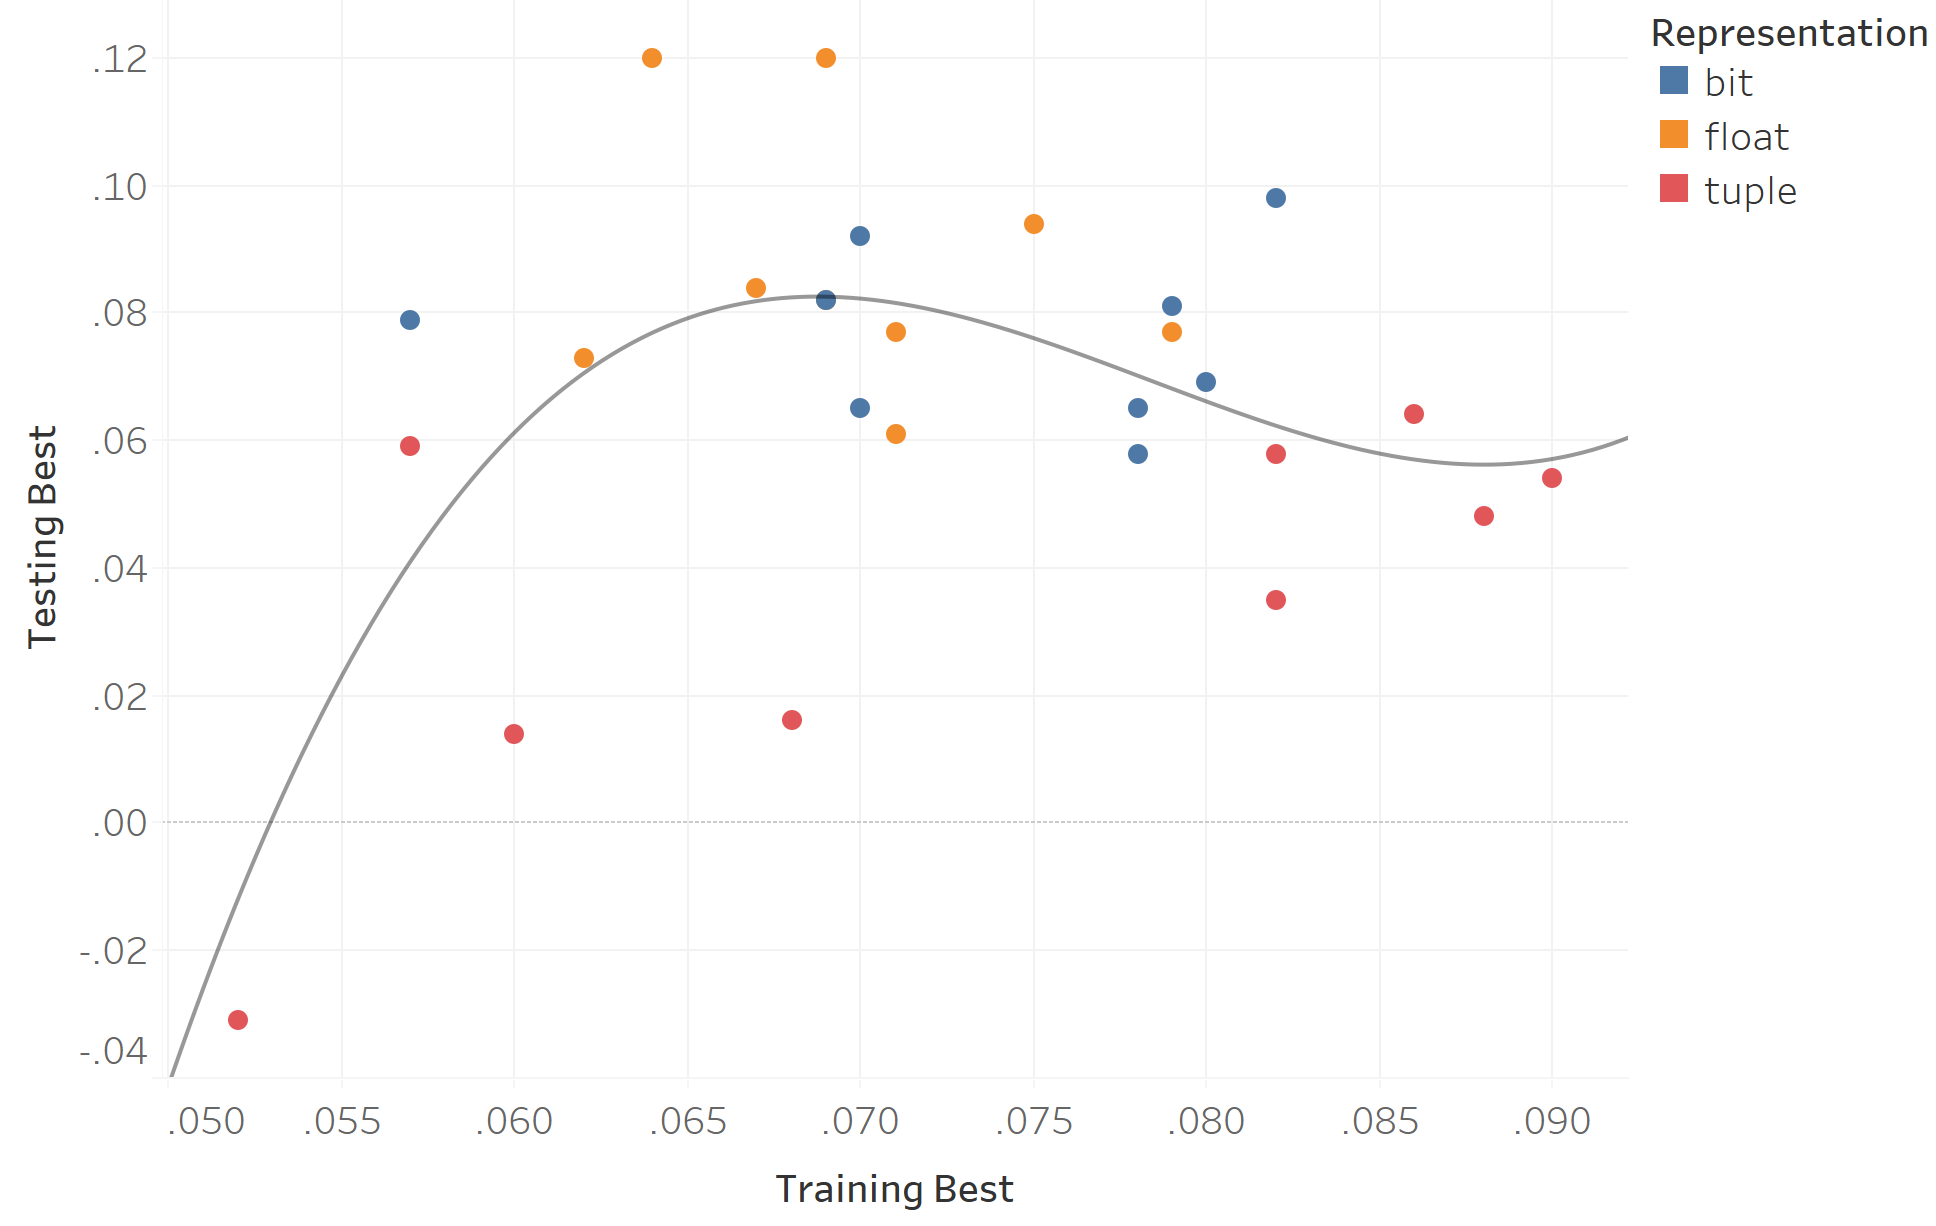
\includegraphics[width=\textwidth]{best.png}
            \subcaption{Training and Testing Best}
        \end{minipage}
        \begin{minipage}[t]{0.49\textwidth}
            \centering
            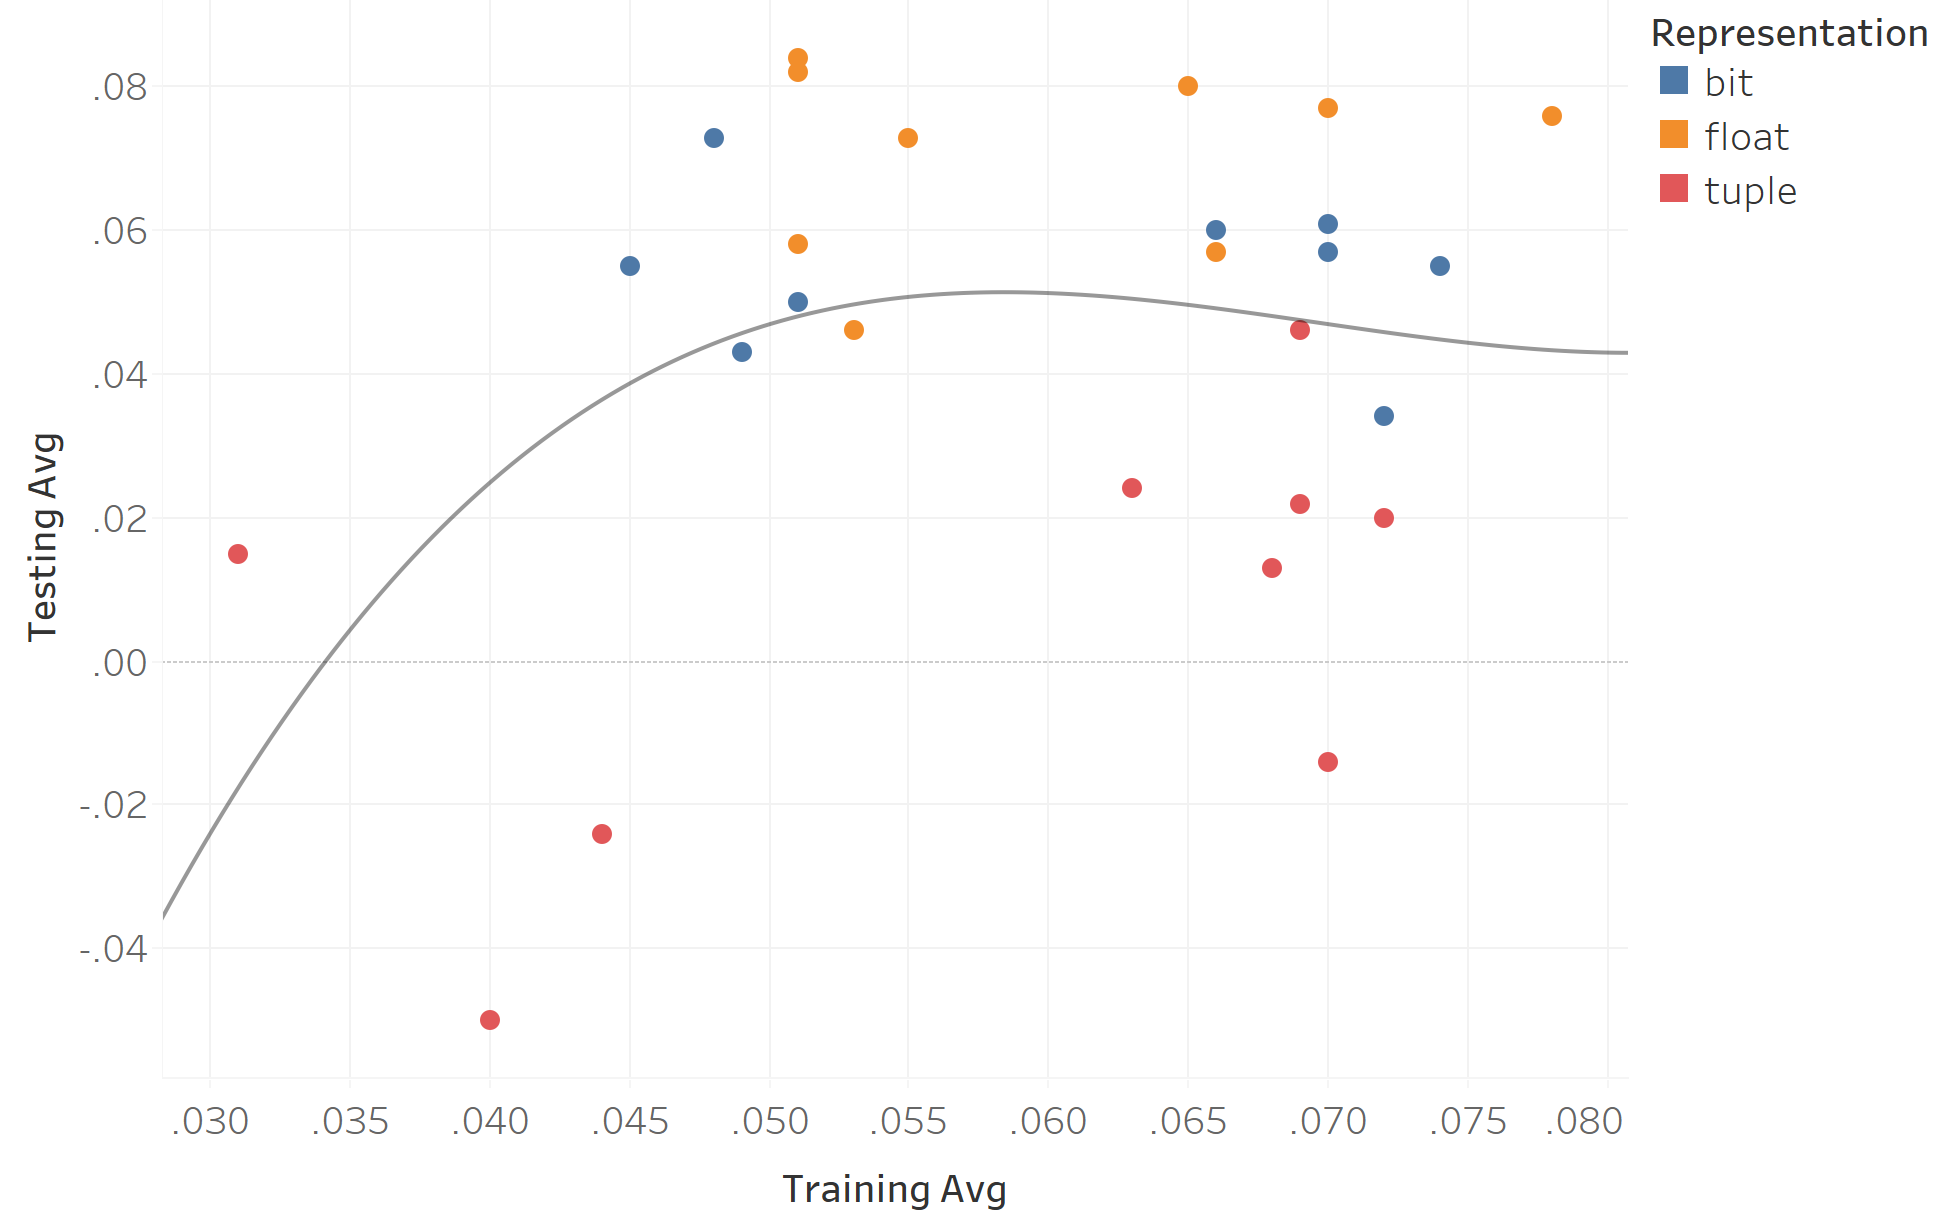
\includegraphics[width=\textwidth]{avg.png}
            \subcaption{Training and Testing Average}
        \end{minipage}
        \caption{Training and Testing Results}
\end{figure}

Both best and average measurements show such a pattern,
that as the training performance improves,
the testing performance will increase firstly then decrease.
It corresponds to the underfitting--optimum--overfitting routine in a lot of machine learning problems.
Blindly pursue a better performance on the train set does not necessarily lead to
a higher profit in the future.
Finding appropriate configuration for the genetic algorithm is critical to building
a successful trading agent that can be put into the real world.

The differences between the chromosome representations once again show an interesting pattern
in this visualization.
Those having the highest test scores are all float represented agents.
The limitation of the flexibility of bit representation constrains its performance
so it can hardly be the best.
On the other hand, although some tuple represented agents can have incredible training performance,
they tend to perform poorly in the test.
Abandoning the benefit of domain knowledge and the overfitting leads to such a result.
The exact configurations of the top 3 testing results are listed in the following table.

\begin{table}[H]
    \centerline{
    \begin{tabular}{ccccc|cc}
    Representation & Survival & Crossover & Mutation & Elitism & Testing Best & Testing Avg \\\hline
    float          & 0.6      & 0.75      & 0.1      &         & 0.12         & 0.084       \\
    float          & 0.6      & 0.75      & 0.1      & 0.1     & 0.12         & 0.082       \\
    bit            & 0.6      & 0.75      & 0.3      &         & 0.098        & 0.043
    \end{tabular}
    }
    \caption{Top 3 Configurations for the Testing Best}
\end{table}


\section{Conclusion and Future Work}

In this research, we successfully used the genetic algorithm to design a trading agent on the stock market.
Besides traditional parameters configuration, we also explored elitism and complex chromosome representation
and examined their effect.
The best agent, which can achieve about 12\% of the theoretically possible revenue on the test market,
is derived with the following genetic algorithm configuration:
\begin{multicols}{2}
\begin{itemize}
    \item Representation: float
    \item Survival rate: 0.6
    \item Crossover rate: 0.75
    \item Mutation rate: 0.1
    \item Elitism: off
    \item Training epoch: 8
\end{itemize}
\end{multicols}

We found in the exploration that chromosome representation makes a huge difference.

Firstly, the same survival/crossover/mutation rate and elitism configuration have
different effects on different representations.
With tuple representation, where the search space is extremely large,
using a high mutation rate or survival rate is likely to cause the best agent's performance to fluctuate
and even stop improving.
Elitism works well to mitigate this problem.
On the contrary, the population of simple bit chromosomes has a tendency to be homogenized.
A higher mutation rate and survival rate is helpful to maintain the gene diversity.

Secondly, the chromosome representation dominantly decides the outcome of the optimization.
The most flexible tuple representation can achieve the highest score on the training dataset.
Nevertheless, the overfitting problem causes an undesirable result on the testing dataset.
The float representation combined the financial domain knowledge and flexibility,
which turns out to perform good enough on the training dataset and the best on the testing dataset.

Some variants of the genetic algorithm are not implemented in our research,
such as adaptive GA and parallel implementation.
Other machine learning techniques, such as support vector machine and neural networks
could be combined to see if they can achieve a better result as well.
Moreover, on the stock market, there are also other problems such as portfolio management and selection,
applying the genetic algorithm in that field could be another interesting topic.
These are the possible further directions based on our works.


\section{Contribution}

YiFan Li:

\begin{itemize}
    \item Read 40\% of the previous literatures
    \item Write all experiment code
    \item Refine \textit{Introduction} and \textit{Related Work}
    \item Write \textit{Abstract, Approach, Results and Analysis, Conclusion, Further Work}
    \item Coordinate works and progress
\end{itemize}

\noindent
ZeYuan Yang:

\begin{itemize}
    \item Read 60\% of the previous literatures
    \item Write first draft of \textit{Introduction} and \textit{Related Work}
    \item Write \textit{Appendix: Financial Rules}
\end{itemize}

\bibliographystyle{abbrv}
\bibliography{report}


\section{Appendix: Financial Rules}\label{section-appendix-financial-rules}

\begin{itemize}

\item Single MA Crossover

\emph{A buy signal is triggered when the Clossing Price Crosses the 28 moveing average to the Upside.}

\emph{A sell signal is triggered when the Clossing Price Crosses the moveing average to the Downside.}
\cite{genetic-algorithms-for-predicting-the-egyptian-stock-market}

\item Double MA Crossover

\emph{MA1 = 25 days}

\emph{MA2 = 50 days}

\emph{A buy signal is triggered when the faster MA1 crosses the slower MA2 to the Upside.}

\emph{A sell signal when the faster MA1 crosses the slower MA2 to the Downside.}
\cite{genetic-algorithms-for-predicting-the-egyptian-stock-market}

\item RSI (relative strength index)

\emph{RS = (An average of upward price movement) / (An average of downward price movement)}

\emph{RSI = 100 - 100 / (1 + RS)} 
\cite{stock-market-prediction-model-using-TPWS}

\item Stochastic Oscillator

\emph{\% k = (Today’s Closing price-lowest low in \% k periods) * 100 / (Highest high in \% k periods-lowest low in \% k periods)}

\emph{\% D= A moving average of \%K is then calculated using the number of time periods specified in the \%D Periods}

\emph{\%k} and \emph{\%D} are two lines Stochastic Oscillator displayed. 
\cite{stock-market-prediction-model-using-TPWS}

\item MA 918

\emph{A buy signal is triggered when the 9 MA crosses the 18 MA to the Upside.}

\emph{A sell signal is triggered when the 9 MA crosses the 18 MA to the Downside.}
\cite{stock-market-prediction-model-using-TPWS}

\item MA 4918

\emph{A buy signal is triggered when the 4 MA crosses the 9 MA to the Upside and the 9 MA crosses the 18 MA to the Upside.}

\emph{A sell signal is triggered when the 9 MA crosses the 18 MA to the Downside.}
\cite{stock-market-prediction-model-using-TPWS}

\item MACD 

\emph{MACD = 7 day Exponential Moving Average - 13 day Exponential Moving Average}
\cite{stock-market-prediction-model-using-TPWS}

\item MFI (money flow index)

\emph{Money Ratio = Positive Money Flow / Negative Money Flow}

\emph{MFI = 100 - 100 / (1 + MR)}
\cite{stock-market-prediction-model-using-TPWS}

\item CCI (commodity channel index)

\emph{Typical Price = (high + low + close) / 3}

\emph{CCI = (Today's Typical Price - Today's 18th period moving average) / (0.015 * Step 3' value)}
\cite{stock-market-prediction-model-using-TPWS}

\item Stochastic RSI

\end{itemize}



%-------%



\end{document}



